% Chapter Template

\chapter{Using a Wind Turbine as a Sensor} % Main chapter title

\label{Chapter2} % Change X to a consecutive number; for referencing this chapter elsewhere, use \ref{ChapterX}


%----------------------------------------------------------------------------------------
%	SECTION 1
%----------------------------------------------------------------------------------------

\section{Introduction}

When using a wind turbine as a sensor, the fundamental questions are: What should we measure, and how should we measure it? In this chapter several possible answers to those questions are investigated. To minimize cost, we will restrict ourselves to using sensors that are already present on a typical wind turbine. This chapter will first evaluate several methods for estimating wind speed, but will also discuss other potentially useful measurements.

There are two advantages to measuring wind speed.  First, both the steady state torque and steady state collective blade pitch are ultimately functions of the incoming wind speed (as shown in Figure \ref{fig2-1}).  Second, the wind speed provides an estimate of the speed at which turbulent eddies in the wind travel. As a result, the wind speed can be used to estimate how long it will take for the wind gusts observed by the upwind turbine to reach the downwind turbine. 


\begin{figure}[htbp]
	\centering
		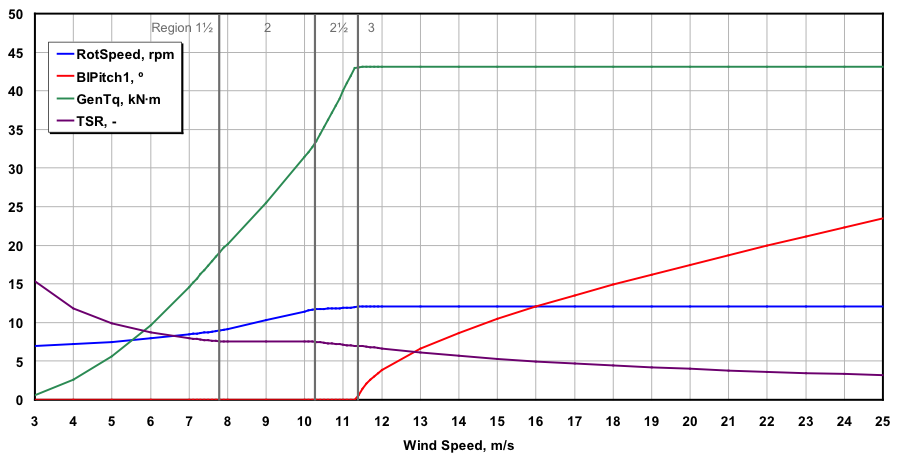
\includegraphics[width=\linewidth]{Figures/ch2Figures/fig2-1.png}
		
	\caption{Steady state rotor speed, blade pitch, generator torque, and tip speed ratio as a function of wind speed for the NREL 5-MW turbine.\cite{jonkman2009}}
	\label{fig2-1}
\end{figure}

Section \ref{section2-2} describes a set of 66 turbulent wind fields. Those wind fields are used in subsequent sections to evaluate sensor techniques. Section \ref{section2-3} discusses wind speed estimates based on nacelle top anemometer readings. Section \ref{section2-4} discusses the use of turbine dynamics for wind speed estimation. Section \ref{section2-5} discusses convection speed estimation, while Section \ref{section2-6} briefly discusses other turbine sensors that could be useful for feed forward control.



%----------------------------------------------------------------------------------------
%	SECTION 2
%----------------------------------------------------------------------------------------

\section{Data for evaluating sensor techniques} \label{section2-2}

The rest of this chapter discusses several wind turbine sensor scheme$'$s that could potentially be used for feed forward control of downwind turbines. To gain insight into the performance of these scheme$'$s, a series of simulations were conducted. The simulations were carried out in FAST (Fatigue, Aerodynamics, Structures, and Turbulence), using wind conditions simulated by TurbSim. FAST is a medium fidelity wind turbine simulation tool developed by NREL and Oregon State University. FAST models both the aerodynamics and structural dynamics of horizontal axis wind turbines, and has been independently validated and verified\cite{manjock2005}. TurbSim is a stochastic, full-field, turbulent-wind simulator. It uses a statistical model (as opposed to a physics based model) to numerically simulate a time series of three-component wind-speed vectors at points on a two-dimensional vertical rectangular grid (see Figure \ref{fig2-2}) \cite{jonkman2012}. All simulations described in this section assumed an NREL 5-MW turbine in great plains low level jet (GPLLJ) wind conditions.

\begin{figure}[htbp]
	\centering
		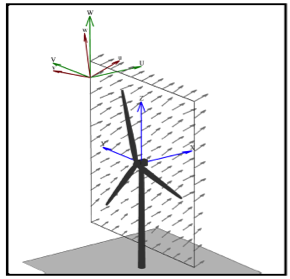
\includegraphics[width=.5\linewidth]{Figures/ch2Figures/fig2-2.png}
		
	\caption{Illustration of TurbSim flow field.\cite{jonkman2012}}
	\label{fig2-2}
\end{figure}

A variety of mean wind speeds were simulated to capture performance over the turbine$'$s whole operating range. Eleven (11) mean wind speeds were simulated ranging from 4 m/s to 24 m/s in 2 m/s increments. At each wind speed 6 unique turbulent wind fields were generated using TurbSim. Each of these wind fields were used to drive a FAST simulation of the NREL 5-MW turbine. Each simulation was 10 minutes long. In total 66 10-minute simulations of an NREL 5-MW turbine in GPLLJ winds were performed.  Sample FAST input files for the simulations can be found in Appendix \ref{AppendixA}.





%----------------------------------------------------------------------------------------
%	SECTION 3
%----------------------------------------------------------------------------------------

\section{Wind speed estimate based on nacelle top \\
anemometer}\label{section2-3}

All utility scale wind turbines have nacelle-mounted anemometers. Anemometer measurements are used for purposes such as assessing wind turbine performance and forecasting future power production. Anemometer measurements are not used by conventional wind turbine control systems, but could potentially be used for wind turbine control.

In some ways, using a nacelle top anemometer is the simplest method to estimate incoming wind speed. The anemometer is designed to measure wind speed. It is located on top of the nacelle, which is near the center of the rotor$'$s swept area. Anemometers and data acquisition system are already in place on all modern utility scale wind turbines. 

However, this method has several complications as well. The anemometer only measures wind speed for a very small portion of the flow field. On modern utility scale wind turbines, where rotors are often more than 100 meters in diameter, the anemometer reading may not be sufficient to accurately represent wind speed across the whole rotor. In addition, suitable anemometer data may not be readily available. For example, the data acquisition system on a Vestas V90 turbine does not provide raw anemometer data. Instead, it provides 10 minute average wind speeds that are based on anemometer data and a proprietary data processing technique. For the sake of this investigation we will assume that raw anemometer data can be obtained, perhaps with the help of the turbine manufacturer.

If suitable anemometer data is available, there may be difficulty obtaining an accurate wind speed measurement. Anemometer data  has high frequency noise and occasional false values. The anemometer could have errors due to poor calibration. In addition, the nacelle top location of the anemometer means it is measuring wind that has passed through the rotor plane. The simulation results shown in Figure \ref{fig2-3} were generated using SOWFA (Simulator fOr Wind Farm Applications), a simulation tool that will be discussed in Chapter \ref{Chapter5}. As Figure \ref{fig2-3} shows, wind in the nacelle area can be significantly affected by the rotor. For the sake of this investigation, we will assume the anemometer data can be processed to obtain an accurate measurement of the incoming wind speed at the center of the rotor.



\begin{figure}[htbp]
	\centering
		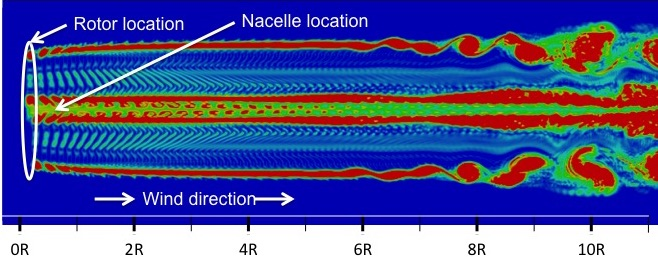
\includegraphics[width = \linewidth]{Figures/ch2Figures/fig2-3.jpg}
		
	\caption{Vorticity downstream of an NREL 5-MW rotor in uniform 11 m/s wind.}
	\label{fig2-3}
\end{figure}





%-----------------------------------
%	SUBSECTION 3-1
%-----------------------------------
\subsection{Feasibility} \label{section2-3-1} 

The simulation data set described in Section \ref{section2-2} was used to evaluate the feasibility of using a nacelle top anemometer to estimate incoming wind speed.  FAST does not simulate the nacelle top anemometer. However, if we make the assumptions stated in the previous two paragraphs we an anemometer would perfectly measure wind speed at the center of the turbine rotor. The  incoming wind speed at the rotor center can be extracted from the TurbSim flow field, and will be treated as the nacelle top anemometer measurement for the remainder of this discussion(Figure \ref{fig2-4}-a). The average wind speed passing through the rotor of the turbine can also be calculated from the TurbSim flow field (Figure  \ref{fig2-4}-b). By comparing these two values we get a feel for how well a nacelle top anemometer can represent the wind passing through the rotor of a utility scale turbine.

\begin{figure}[htbp]
	\centering
		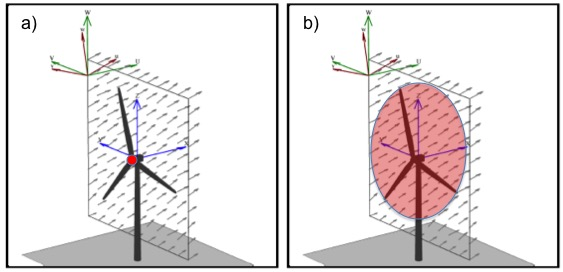
\includegraphics[width = \linewidth]{Figures/ch2Figures/fig2-4.jpg}
		
	\caption{Measurement locations for the rotor center wind speed and rotor average wind speed.}
	\label{fig2-4}
\end{figure}

Figure \ref{fig2-6} shows wind speed at the anemometer as well as the average wind speed across the swept area of the rotor. The data shown in the figure is from the 13th simulation in the data set described above, but this data is typical of the other 65 simulations as well. At first glance the anemometer wind speed looks noisy compared to the rotor average wind speed. Upon closer examination (Figure \ref{fig2-7}) we see that both the anemometer and the rotor average wind speed have high frequency fluctuations. However, the high frequency fluctuations in the anemometer wind speed have a much larger magnitude. 

\begin{figure}[htbp]
	\centering
		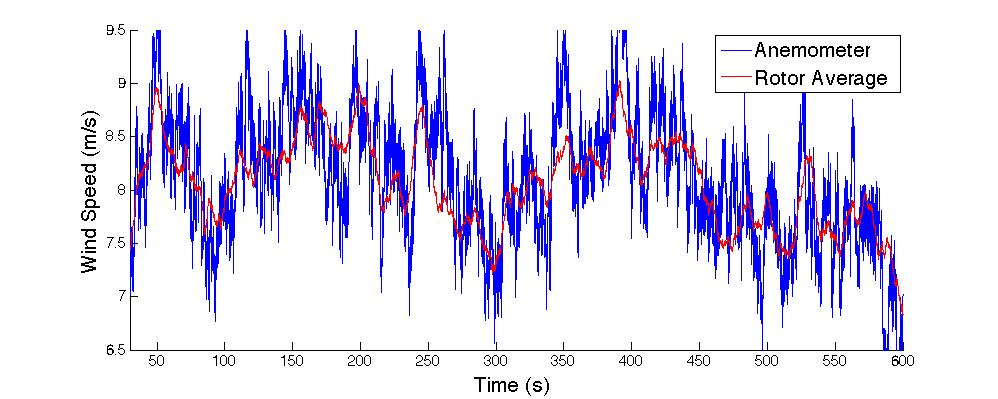
\includegraphics[width = \linewidth]{Figures/ch2Figures/fig2-6.jpg}
		
	\caption{Anemometer measurement and rotor average wind speed for simulation \#13 (8 m/s average wind speed).}
	\label{fig2-6}
\end{figure}


\begin{figure}[htbp]
	\centering
		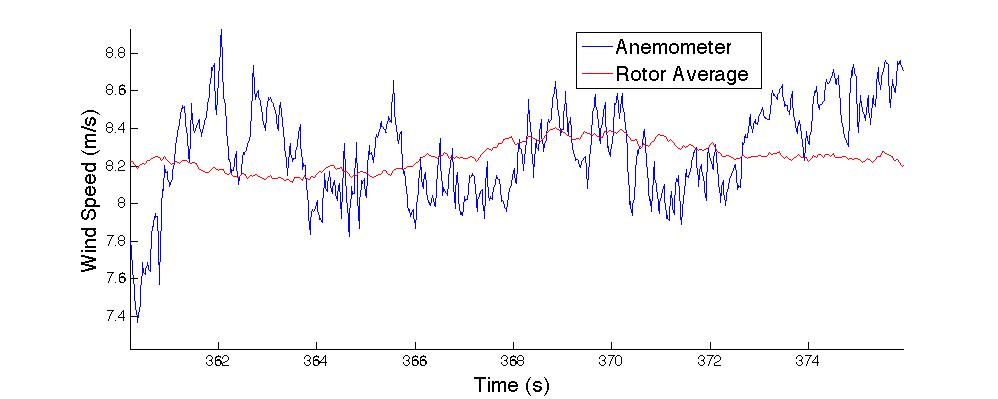
\includegraphics[width = \linewidth]{Figures/ch2Figures/fig2-7.jpg}
	\caption{Zooming in on Figure \ref{fig2-6} shows high frequency oscillations are present in both anemometer measurements and rotor average wind speed.}
	\label{fig2-7}
\end{figure}

The magnitude of these high frequency fluctuations is not very important from a wind turbine control point of view. Because utility scale wind turbines are such large machines, it isn$'$t practical for the blade pitch and generator torque to track high frequency fluctuations in wind speed. In a typical utility scale turbine controller feedback signals are passed through a low pass filter before they are used for turbine control. To get a more meaningful comparison between anemometer wind speed and rotor average wind speed we should filter out the high frequency fluctuations.

Figure \ref{fig2-8} shows anemometer wind speed and rotor average wind speed from simulation \#13 after they have been passed through a low pass filter. I chose to use a 4th order zero-phase filter with a 0.25 Hz cutoff frequency. A zero phase filter was chosen because it does not result in a delay of the filtered signal. A 0.25 Hz cutoff frequency was chosen because it is the corner frequency of the low pass filter used by the NREL 5-MW control system. 

\begin{figure}[htbp]
	\centering
		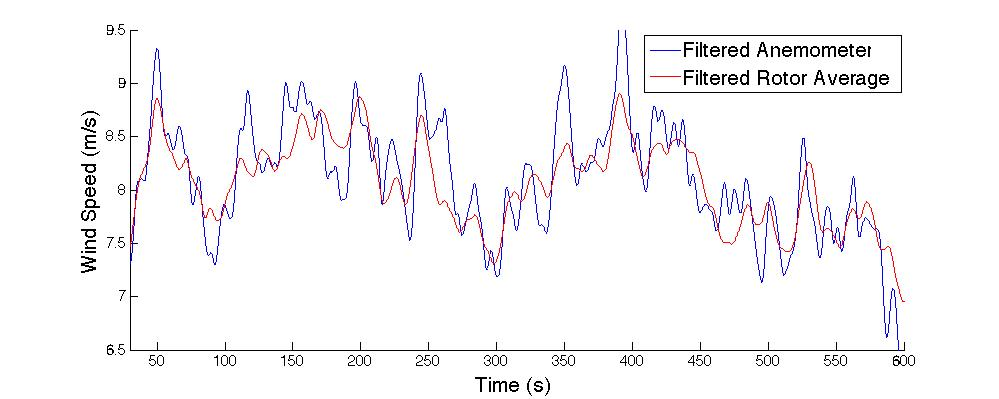
\includegraphics[width = \linewidth]{Figures/ch2Figures/fig2-8.jpg}
		
	\caption{Filtered anemometer and rotor average wind speed for simulation \#13.}
	\label{fig2-8}
\end{figure}

Figure \ref{fig2-9} shows the discrepancy between the filtered anemometer wind speed and the filtered rotor average wind speed for simulation \#13. For this run the magnitude of the discrepancy ranges from almost 0 to as much as 0.954 m/s, and the average magnitude of the discrepancy is 0.236 m/s. All 6 simulations run with an 8 m/s wind speed yield similar data, as can be seen in Figure \ref{fig2-10}. Between these 6 simulations there are 57 minutes of data. If the magnitudes of the discrepancies are averaged over all data points in these 6 simulations, we find the discrepancy between the filtered anemometer wind speed and the filtered rotor average wind speed averages 0.272 m/s when the NREL 5-MW turbine is in 8 m/s GPLLJ wind conditions.

\begin{figure}[htbp]
	\centering
		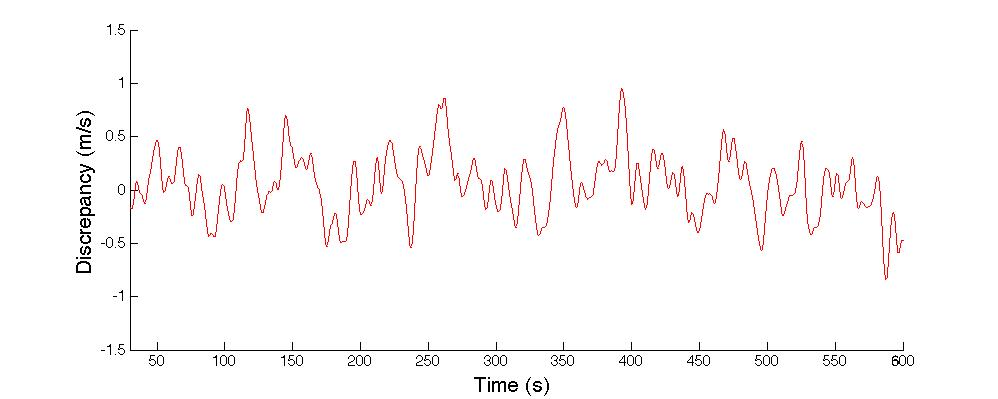
\includegraphics[width = \linewidth]{Figures/ch2Figures/fig2-9.jpg}
		
	\caption{Discrepancy between anemometer and rotor average wind speed for simulation \#13.}
	\label{fig2-9}
\end{figure}

\begin{figure}[htbp]
	\centering
		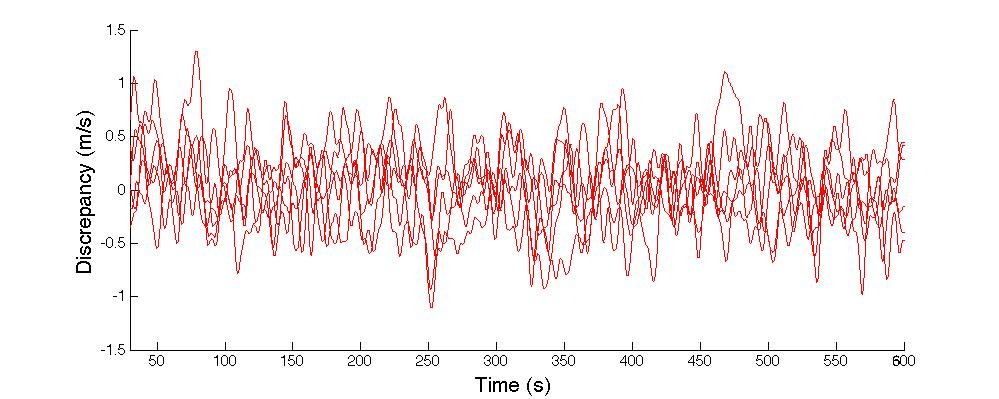
\includegraphics[trim = {.25cm 0 2.5cm 0}, clip, width = .95\linewidth]{Figures/ch2Figures/fig2-10.jpg}
		
	\caption{Discrepancy between anemometer and rotor average wind speed for all 8 m/s simulations.}
	\label{fig2-10}
\end{figure}


Repeating that process for all the mean wind speeds simulated in the data set yields Figure \ref{fig2-11} and Figure \ref{fig2-12}. Figure \ref{fig2-11} shows average magnitudes of the discrepancies between anemometer wind speed and rotor average wind speed in m/s, while Figure \ref{fig2-12} shows the same quantity expressed as a percentage the mean wind speed. Each * on the plot represents an average over all 57 minutes of simulation data at the corresponding wind speed. Figure \ref{fig2-11} shows that the smallest average discrepancy is 0.269 m/s, which occurs at a mean wind speed of  6 m/s. When we examine the discrepancy as a percentage of the mean free stream wind speed  (Figure \ref{fig2-12}) we see that the average discrepancy is approximately 3\% of the mean wind speed over most of the operating range of the NREL 5-MW turbine, though the  average discrepancy is a larger percentage at low wind speeds.

\begin{figure}[htbp]
	\centering
		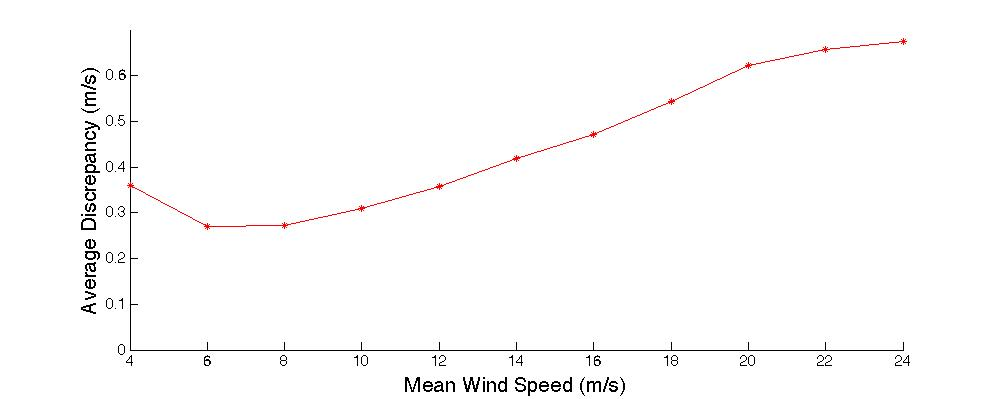
\includegraphics[width = \linewidth]{Figures/ch2Figures/fig2-11.jpg}
		
	\caption{Average magnitude of discrepancy (in m/s) as a function of simulation mean wind speed.}
	\label{fig2-11}
\end{figure}

\begin{figure}[htbp]
	\centering
		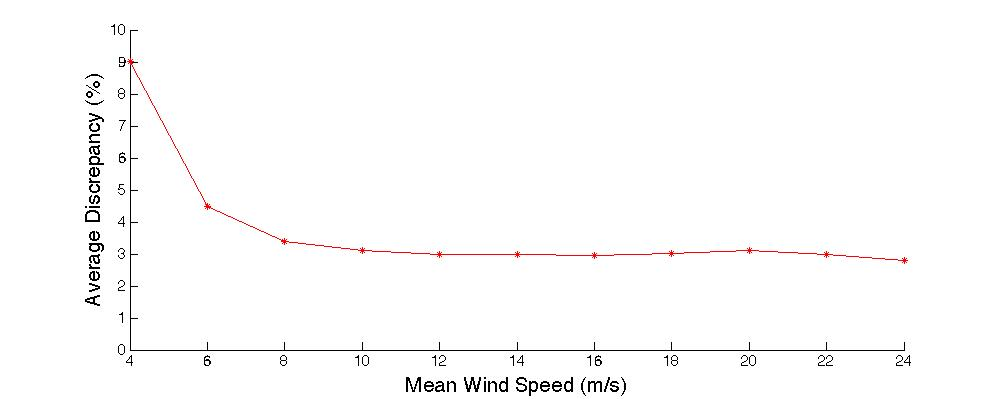
\includegraphics[width = \linewidth]{Figures/ch2Figures/fig2-12.jpg}
		
	\caption{Average magnitude of discrepancy (in \%) as a function of simulation mean wind speed.}
	\label{fig2-12}
\end{figure}



%----------------------------------------------------------------------------------------
%	SECTION 4
%----------------------------------------------------------------------------------------

\section{Turbine Model Based Wind Speed Estimator} \label{section2-4} 

Incoming wind speed can also be estimated using an inverted dynamic model of the turbine.  First the generator speed, generator torque, and pitch angle are measured.  The inverted model is then used to determine the mean incoming wind speed that would cause the observed turbine operating conditions.  In effect, the turbine itself is used as a wind speed sensor. \cite{ostergaard2007,vanderhooft2004,schlipf2014}

We begin with a simplified model of the wind turbine in which the only degrees of freedom are the rotational speed of the rotor ($\Omega _{Rotor}$), the collective blade pitch ($\theta$), and the torque supplied by the generator ($T_{Gen}$).  The dynamics of the turbine are given by equation \ref{eq2-1}, where $I_{Drivetrain}$ is the low speed shaft equivalent inertia, $T_{Aero}$ is the aerodynamic torque on the rotor, and $N_{Gear}$ is the gear box ratio:

\begin{equation}
	\dot{\Omega }_{Rotor}I_{Drivetrain}=T_{Aero}-T_{Gen}N_{Gear} \label{eq2-1}
\end{equation}

Essentially, equation  \ref{eq2-1} says the rotational acceleration of the rotor multiplied by the effective inertia of the rotor is equal to the sum of the torques applied to the rotor. The low speed shaft equivalent inertia ( $I_{Drivetrain}$) is the rotational inertia of the rotor plus the apparent inertia due other components of the drivetrain. It can be calculated from the rotational inertias of the drivetrain components and the gearbox ratio ($N_{Gear}$). There are two torques applied to the rotor. The torque exerted by the generator is equal to the generator torque multiplied by the gearbox ratio. The aerodynamic torque exerted on the rotor by the incoming wind ($U$) is given by equation \ref{eq2-2}, where $\rho$ is is air density, $R$ is the rotor radius, $C_p$ is the coefficient of power, and $\lambda$ is the tip speed ratio:

\begin{equation}
	T_{Aero}=\frac{1}{2}\rho R^{3}\frac{C_{p}(\lambda,\theta)}{\lambda}U^{2} \label{eq2-2}
\end{equation}

The tip speed ratio $\lambda$ is the ratio between the speed of the turbine blade tips and the speed of the incoming wind. It can be calculated using equation \ref{eq2-3}. The coefficient of power $C_p$ is a non-linear function of both tip speed ratio and collective blade pitch angle. A method for determining $C_p$ will be discussed below

\begin{equation}
	\lambda=\frac{\Omega_{Rotor} R}{U} \label{eq2-3}
\end{equation}

Equation \ref{eq2-2} has four quantities that are not directly measurable: $T_{Aero}$, $C_p,$ $\lambda$, and $U$. If equation \ref{eq2-1} is used to substitute for $T_{Aero}$ equation \ref{eq2-2} becomes:

\begin{equation}
	\dot{\Omega }_{Rotor} I_{Drivetrain} + T_{Gen} N_{Gear} = \frac{1}{2} \rho R^3 \frac{C_p ( \lambda , \theta )}{\lambda} \left(\frac{\Omega_{Rotor} R}{\lambda}\right)^2   \label{eq2-4}
\end{equation}

Which can be re-arranged to yield equation \ref{eq2-5}. All the terms on the right side of equation \ref{eq2-5} are known or easily measured from sensors on the wind turbine. Therefore, equation \ref{eq2-5} can be used to calculate $C_p / \lambda^3$.

\begin{equation}
	 \frac{C_p ( \lambda, \theta)}{\lambda^3} = \frac{2 \dot{\Omega}_{Rotor} I_{Drivetrain} + 2 T_{Gen} N_{Gear}}{\rho R^5 \Omega^2_{Rotor}} \label{eq2-5}
\end{equation}


The coefficient of power $C_p$ is a non-linear function of both tip speed ratio and collective blade pitch angle. It isn$’$t possible to calculate $C_p$ exactly, but for a given tip speed ratio and collective blade pitch it is possible to estimate the $C_p$ of a turbine through simulation.  Figure \ref{fig2-13} illustrates how $C_p$ of the NREL 5-MW turbine varies with $\lambda$ and collective blade pitch angle (in \degree). This plot was generated from a large number of simulations carried out with WTPerf \cite{platt2012}. Note that the maximum $C_p$ corresponds to a 0\degree collective pitch angle and a tip speed ratio of 7.55. The turbine operates near this point when using variable speed control in region 2. 

\begin{figure}[ht]
	\centering
		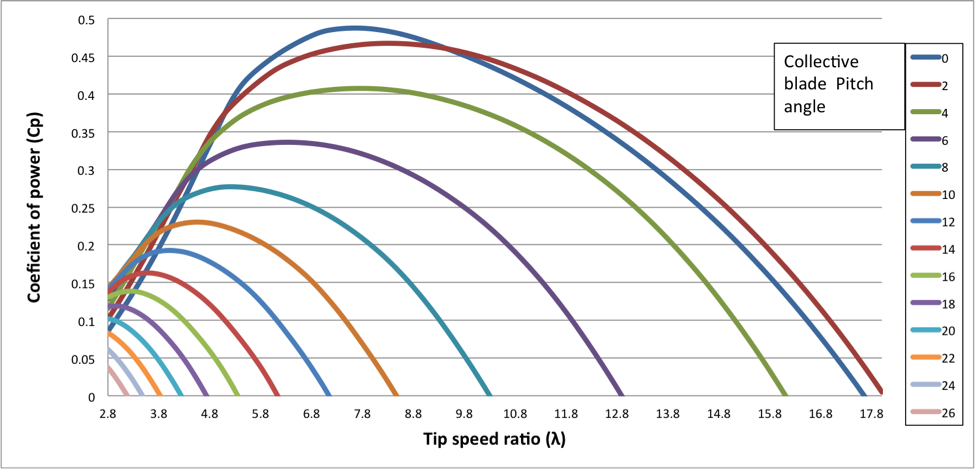
\includegraphics[width=\textwidth]{Figures/ch2Figures/fig2-13.png}
		
	\caption{$C_p$ dependence on $\lambda$ and collective blade pitch angle (\degree).}
	\label{fig2-13}
\end{figure}

The collective pitch angle is measured by turbine sensors, but both $C_p$ and $\lambda$ are unknown quantities that can not be directly measured or easily calculated. However, this problem can be fixed. If each $C_p$ value estimated by WTPerf is divided by the corresponding $\lambda$ cubed we get a relationship between $C_p\lambda^3, \lambda$, and collective pitch angle. Figure \ref{fig2-14}  illustrates how $C_p / \lambda^3$ of the NREL 5-MW turbine varies with $\lambda$ and collective blade pitch angle (in \degree). 

\begin{figure}[ht]
	\centering
		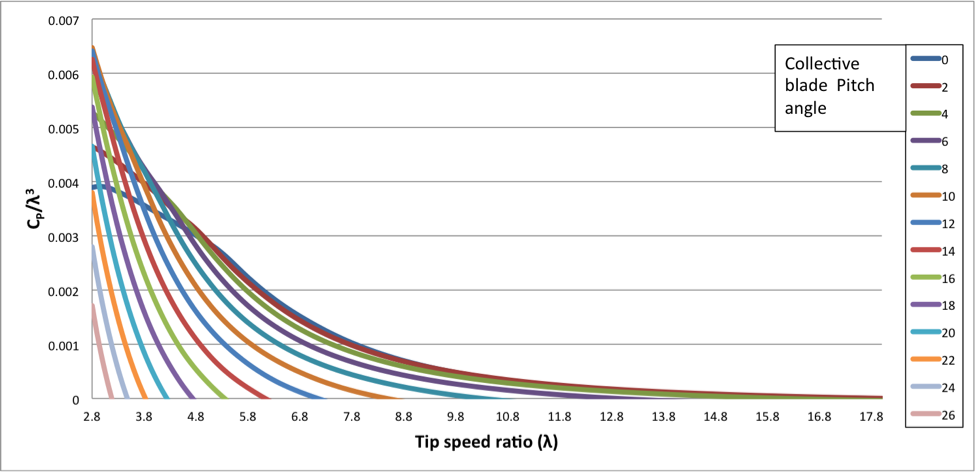
\includegraphics[width=\textwidth]{Figures/ch2Figures/fig2-14.png}
		
	\caption{$C_p / \lambda^3$ dependence on $\lambda$ and collective blade pitch angle (\degree).}
	\label{fig2-14}
\end{figure}

The incoming wind speed can now be estimated. First the collective pitch angle is measured and $C_p / \lambda^3$ is calculated using equation \ref{eq2-5}. $\lambda$ is then estimated by interpolating between the WTPerf simulation data points illustrated in Figure \ref{fig2-14}. Finally, $\lambda$ is converted to incoming wind speed ($U$) using equation \ref{eq2-3}. 


%-----------------------------------
%	SUBSECTION 4-1
%-----------------------------------
\subsection{Feasibility} \label{section2-4-1} 

The feasibility of using a turbine model based wind speed estimator was evaluated using similar methods to those used in Section \ref{section2-3-1}. We begin by comparing the average wind speed passing through the rotor of the turbine (calculated from the TurbSim flow field) to the wind speed estimated by the model based wind speed estimator.  This gives us a feel for how well the estimator represents the wind passing through the rotor of a utility scale turbine.

The data in Figure \ref{fig2-15} is from the 13th simulation in the data set described above (the same simulation shown in Figure \ref{fig2-6}), but this data is typical of the other 65 simulations as well. The figure shows that the wind speed estimator is ``noisier'' than the rotor average wind speed. In this way it$'$s similar to the nacelle anemometer measurements shown in Figure \ref{fig2-6}. However, the high frequency fluctuations in the wind speed estimator are smaller than the high frequency fluctuations in the anemometer measurements. 

\begin{figure}[htbp]
	\centering
		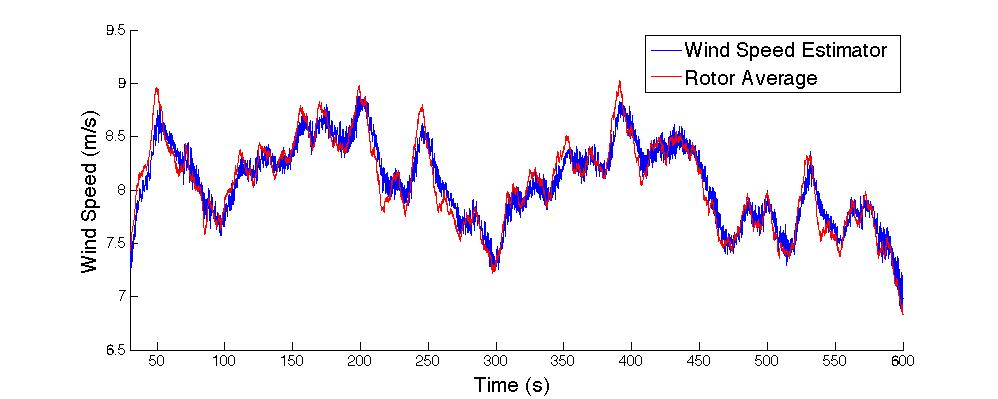
\includegraphics[width = \linewidth]{Figures/ch2Figures/fig2-15.jpg}
		
	\caption{Wind speed estimate and rotor average wind speed for simulation \#13.}
	\label{fig2-15}
\end{figure}


Filtering the data in Figure \ref{fig2-15} to remove the high frequency fluctuations yields Figure \ref{fig2-16}. The wind speed estimator doesn$'$t match the rotor average wind speed perfectly, but a comparison between Figure \ref{fig2-8} and Figure \ref{fig2-16} shows that the wind speed estimator does a much better job than the nacelle top anemometer. This conclusion is reinforced by comparing Figure \ref{fig2-9} to Figure \ref{fig2-17}.

\begin{figure}[ht]
	\centering
		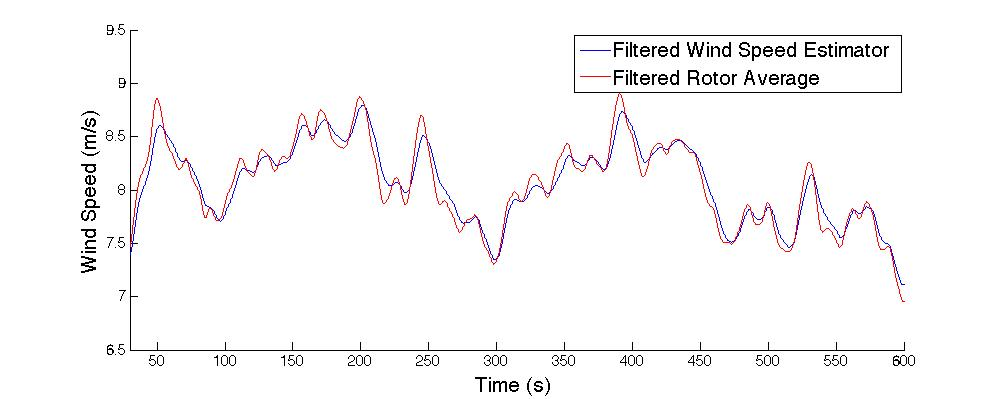
\includegraphics[width = \linewidth]{Figures/ch2Figures/fig2-16.jpg}
		
	\caption{Filtered wind speed estimate and rotor average wind speed for simulation \#13.}
	\label{fig2-16}
\end{figure}



\begin{figure}[ht]
	\centering
		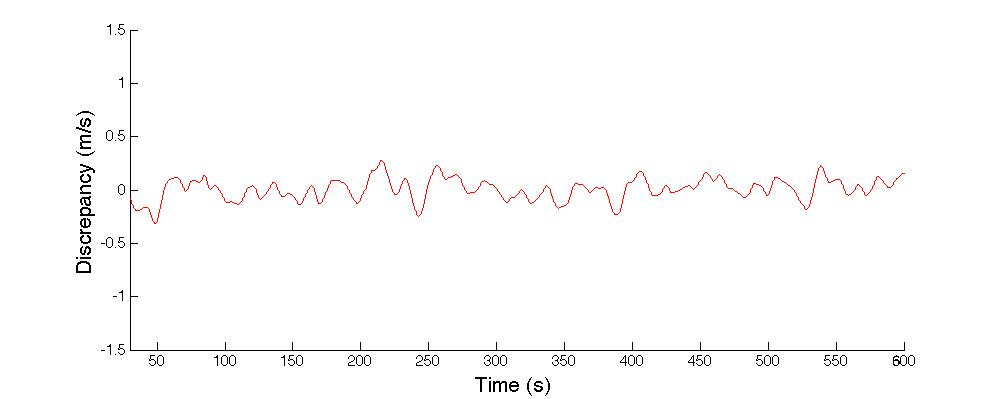
\includegraphics[width = \linewidth]{Figures/ch2Figures/fig2-17.jpg}
		
	\caption{Discrepancy between wind speed estimate and rotor average wind speed for simulation \#13.}
	\label{fig2-17}
\end{figure}

The data shown in Figures \ref{fig2-15}-\ref{fig2-17} are from a single simulation, but the data and the conclusions drawn from it are typical of all the simulation data examined. The wind speed estimator performed significantly better than the nacelle top anemometer. If we analyze the wind speed estimator data for all 66 simulations using the same process used to create Figure \ref{fig2-11} and Figure \ref{fig2-12} we can get an idea of how much better the wind speed estimator performs. Figure \ref{fig2-18} and Figure \ref{fig2-19} compare the average discrepancy between the wind speed estimator and the rotor average wind speed to the average discrepancy between the nacelle top anemometer and the average wind speed. It can be seen from these figures that the wind speed estimator outperforms the anemometer across the entire operating range of the turbine. 


\begin{figure}[ht]
	\centering
		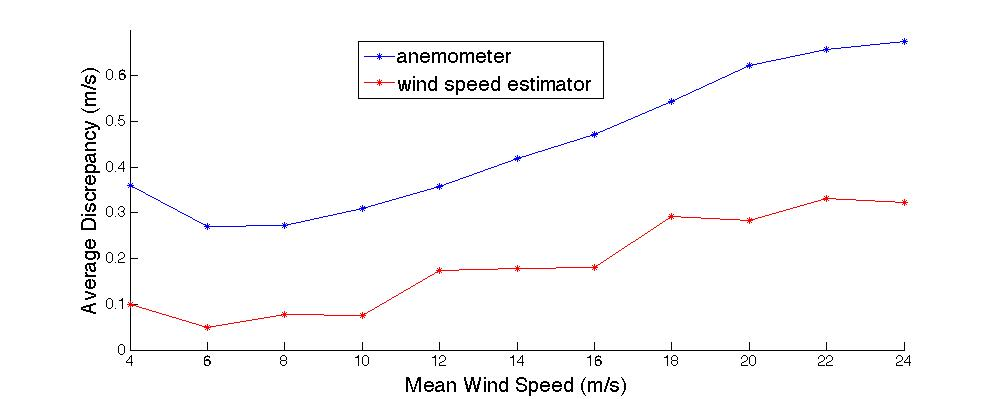
\includegraphics[width = \linewidth]{Figures/ch2Figures/fig2-18.jpg}
		
	\caption{Average magnitude of discrepancy as a function of simulation mean wind speed.}
	\label{fig2-18}
\end{figure}



\begin{figure}[ht]
	\centering
		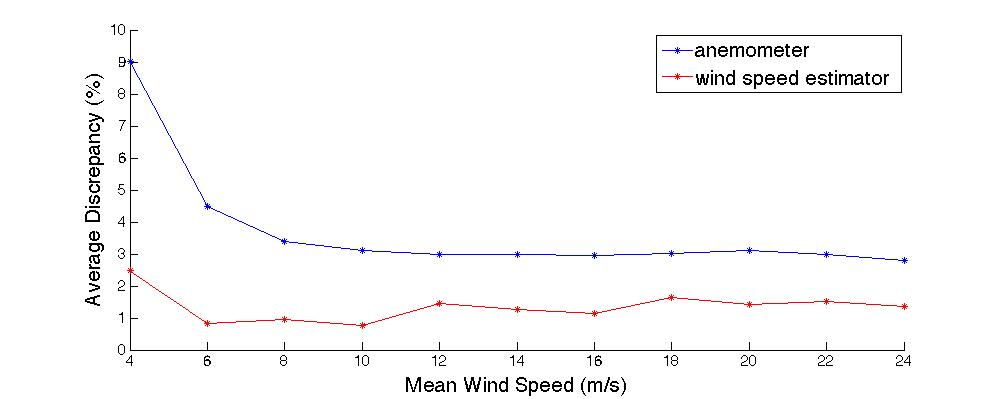
\includegraphics[width = \linewidth]{Figures/ch2Figures/fig2-19.jpg}
		
	\caption{Average magnitude of discrepancy as a function of simulation mean wind speed.}
	\label{fig2-19}
\end{figure}


%-----------------------------------
%	SUBSECTION 4-2
%-----------------------------------
\subsection{Effect of rotor yaw misalignment}\label{section2-4-2} 

The simulations analyzed in the previous sections assume the turbine is pointed directly into the wind. However, in normal turbine operation there is often some misalignment between the wind direction and the pointing direction, or yaw, of the turbine. It is possible to design a turbine that is stable in yaw and will point itself into the wind without the help of a control system or actuators, but in practice this passive control technique is only used for very small turbines. Modern utility scale turbines use active yaw control \cite{burton2011}.

The yaw control on a typical utility scale turbine uses a dead band controller with a nacelle mounted wind vane as a sensor and a nacelle yaw motor as an actuator \cite{burton2011}. In this control scheme the signal from the nacelle mounted wind vane is heavily averaged to reduce the effect of small brief changes in wind direction and to reduce the effect of the turbulence generated by the turbine rotor. That averaged wind vane measurement is then treated as an estimate of the wind direction. The dead band controller compares the wind direction estimate to the current yaw of the turbine. If the misalignment is smaller than a pre-defined limit the controller does nothing, but if the misalignment exceeds the limit the controller engages the yaw motor and yaws the turbine into alignment with the wind. Since the NREL 5-MW turbine does not define a yaw control system, we will assume our turbine uses dead band control.

The amount of misalignment allowed by the dead band yaw controller will vary from one turbine to another. To evaluate the effect of yaw misalignment on wind speed estimation, misalignments of 5\degree, 10\degree, 15\degree, and 20\degree were simulated. For each of these yaw misalignments the 66 test cases described above were simulated.

Figure \ref{fig2-20} shows the effect of rotor misalignment on wind speed estimation for simulation case \#13. As misalignment angle increases the wind speed estimator underestimates wind speed. For 5\degree and 10\degree misalignments this effect appears small, but the effect is much larger for 15\degree and 20\degree misalignments. It$'$s worth noting that the shapes of the wind speed estimate curves do not change much with increasing rotor misalignment. The misalignment primarily affects the magnitude of the wind speed estimates. 


\begin{figure}[ht]
	\centering
		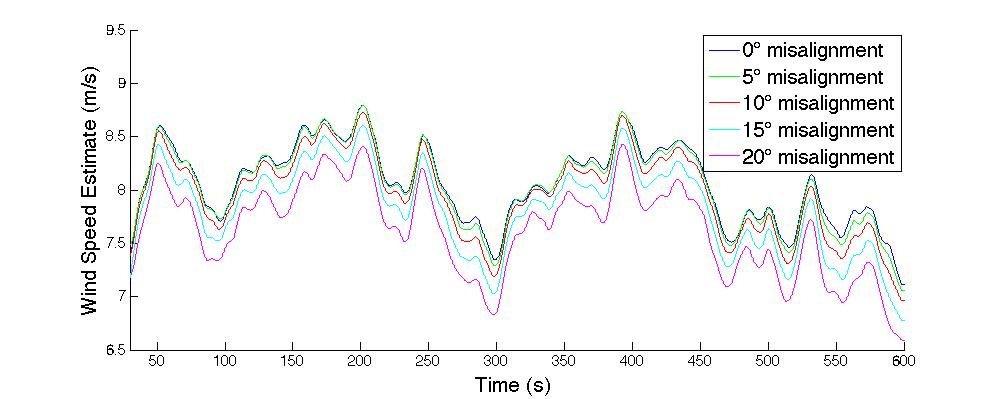
\includegraphics[width = \linewidth]{Figures/ch2Figures/fig2-20.jpg}
		
	\caption{Effect of rotor misalignment on wind speed estimate for simulation \#13.}
	\label{fig2-20}
\end{figure}

Though the data shown in Figure \ref{fig2-20} is from a single simulation case the conclusions drawn from it are typical of all simulation data that was examined. If we analyze the wind speed estimator data for all simulations cases using the same process used to generate Figure \ref{fig2-12}, we can get an idea of how rotor misalignment affects wind speed estimation error. As we saw in Figure \ref{fig2-20} a misalignment of 5\degree or 10\degree causes only a small increase in the discrepancy between estimated wind speed and average rotor wind speed. Larger misalignments cause significantly larger discrepancies. It is worth noting only the 20\degree misalignment performs worse than the nacelle top anemometer (Figure \ref{fig2-12}).

\begin{figure}[ht]
	\centering
		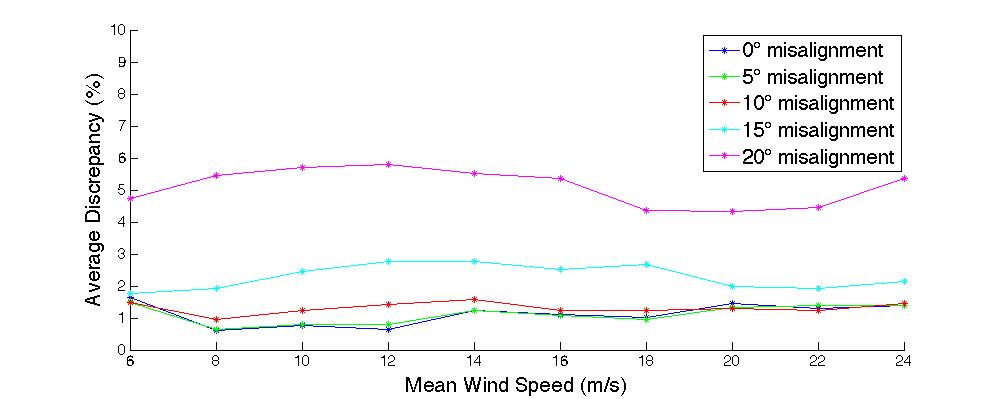
\includegraphics[width = \linewidth]{Figures/ch2Figures/fig2-21.jpg}
		
	\caption{Effect of misalignment on average magnitude of wind speed estimate discrepancy.}
	\label{fig2-21}
\end{figure}


It should not be surprising that a misaligned rotor underestimates wind speed. Our wind speed estimator is based on a simplified model of turbine rotor dynamics. Since wind parallel to the rotor plane does not exert an aerodynamic torque on the rotor our estimator does not measure that component of the wind. Essentially, our wind speed estimator is designed to measure the component of the wind that is perpendicular to the rotor plane. As Figure \ref{fig2-22} shows, the apparent wind seen by the wind speed estimator is equal to the actual wind multiplied by the cosine of the misalignment angle.

\begin{figure}[htbp]
	\centering
		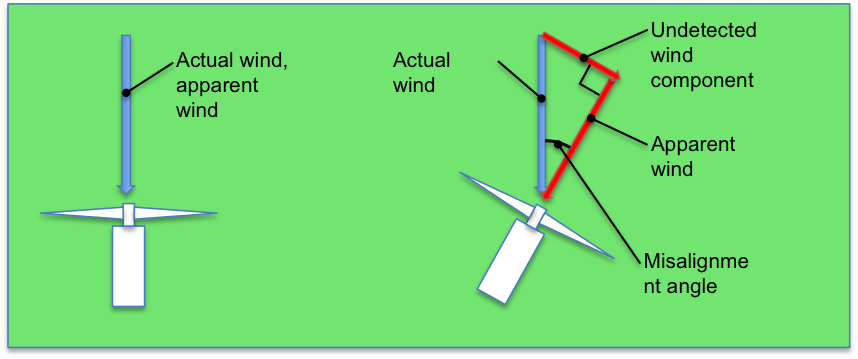
\includegraphics[width=\textwidth]{Figures/ch2Figures/fig2-22.png}
		
	\caption{Effect of rotor misalignment on apparent wind.}
	\label{fig2-22}
\end{figure}

If the misalignment angle is known, it can be used to compensate for the difference between the apparent wind seen by the estimator and the actual wind. If the wind speed estimates shown in Figure \ref{fig2-20} are divided by the cosine of the misalignment angle it yields Figure \ref{fig2-23}. As the figure shows, the effect of misalignment on wind speed estimation has been greatly reduced. 


\begin{figure}[htbp]
	\centering
	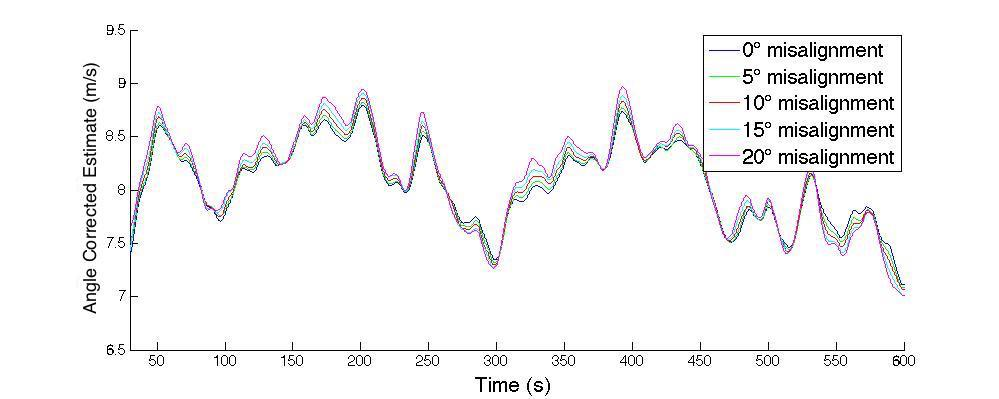
\includegraphics[width = \linewidth]{Figures/ch2Figures/fig2-23.jpg}
		
	\caption{Angle corrected wind speed estimates for simulation \#13.}
	\label{fig2-23}
\end{figure}


Figure \ref{fig2-24} shows the average discrepancy between misalignment-compensated wind speed estimates and rotor average wind speed. The misaligned simulations generally show more discrepancy than the perfectly aligned simulations. However, comparing Figure \ref{fig2-21} to Figure \ref{fig2-24} shows that misalignment compensation greatly reduces the discrepancy. In the 20\degree misalignment simulations the average discrepancy is reduced 60-75\% by angle compensation.


\begin{figure}[htbp]
	\centering
		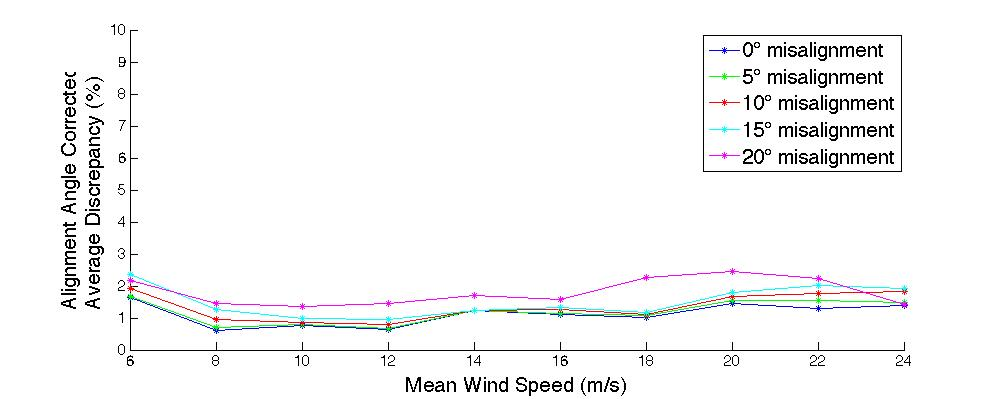
\includegraphics[width = \linewidth]{Figures/ch2Figures/fig2-24.jpg}
		
	\caption{Average magnitude of discrepancy in angle corrected wind speed estimates.}
	\label{fig2-24}
\end{figure}


Though the misalignment angle will not be perfectly known, an estimate of the misalignment angle will be available and can be used for compensation. As stated earlier in this section, the dead band yaw controller continuously estimates the misalignment angle but doesn$'$t act unless the misalignment exceeds a pre-defined limit. 

Yaw misalignment does have an effect on turbine model based wind speed estimation, but it does not appear that it will be a significant hindrance to using turbine model based wind speed estimation. Misalignments less than 10\degree only have a minor effect on performance. Larger misalignments do have a significant effect on performance, but it should be possible to reduce the effect by using misalignment angle compensation.





%----------------------------------------------------------------------------------------
%	SECTION 5
%----------------------------------------------------------------------------------------

\section{Convection speed estimation} \label{section2-5}

The previous sections have discussed instantaneous wind speed estimation. These wind speed estimates can be used to observe how the wind speed is fluctuating as it passes through a wind turbine rotor. However, knowledge of how the wind speed is fluctuating is not sufficient information for feed forward control of downwind turbines. We must also know when these wind speed fluctuations will reach the downwind turbine. The time required for the wind speed fluctuations to pass from the upwind turbine to the downwind turbine can be calculated with the simple equation $t = D/U_{conv}$, where $D$ is the downwind distance between the turbines and $U_{conv}$ is the convection speed. The convection speed is the rate at which wind speed fluctuations propagate downwind. This section will discuss using a wind turbine to estimate the convection speed.

If we assume Taylor's frozen turbulence hypothesis we can estimate the convection speed based on wind speed measurements taken at a single location. In this secion the convection speed will be estimated using the turbine model based wind speed estimates discussed in Section \ref{section2-4}. Taylor said ``If the speed of the air stream which carries the eddies is very much greater than the turbulence speed, one may assume that the sequence of changes in u at a fixed point are simply due to the passage of an unchanging pattern of turbulent motion over the point.'' \cite{taylor1938} In other words, the wind experienced by a point down wind of our sensor will be the same as the wind experienced by the sensor but it will be delayed by a time $t_D = (distance)/(U_{conv})$. It follows from Taylor's hypothesis that the convection speed of the turbulent fluctuations is equal to the local mean speed ($U_{mean}$). 

There is much research into the validity and limitations of Taylr's frozen turbulence hypothesis for estimating the convection speed. \cite{dennis2008,goldschmidt1981,delalamo2009,atkinson2015} Though research shows that the convection speed is not always equal to the mean speed they are frequently assumed to be equal in turbulent flow research. $U_{conv} = U_{mean}$ will be assumed for the remainder of this section. A more accurate estimate of the convection speed could be generated using more than one wind speed measurement location. For example, we could measure the time it took a gust of wind to travel between two turbines. However, this technique can not be used with the data set described in Section \ref{section2-2} because FAST only simulates a single turbine.

For the data set described in Section \ref{section2-2} the mean speed ($U_{mean}$) is known. $U_{mean}$ is one of the TurbSim input parameters used to generate the data set. As shown in equation \ref{eq2-6} we can consider the wind passing through the turbine rotor to be a combination of the underlying mean wind sped ($U_{mean}$) and the wind speed fluctuations due to turbulence ($U_{turb}$). If we average the hub height wind speed over a long enough time the wind speed fluctuations due to turbulence will cancel out and we'll be left with the mean wind speed. 


\begin{equation}
	 U =  U_{mean} +U_{turb}  \label{eq2-6}
\end{equation}

Figure \ref{fig2-25} shows the wind speed estimate, the sixty second average wind speed, and the true mean wind speed for simulation \#13. The wind speed estimate is generated using the method described in section \ref{section2-4}. 60 second average values are generated by averaging 60 seconds of wind speed estimate data (from 30 seconds before to 30 seconds after the time of interest). The true mean wind speed is known and was specified as an input when simulating the incoming wind. There are two things worth noting in Figure \ref{fig2-25}. First, there are significant discrepancies between the 60 second average wind speed and the known mean wind speed of 8 m/s. At 182 seconds there is a 0.587 m/s, or 7.3\%,  discrepancy between the 60 second average wind speed and the true mean wind speed. Also, the 60 second average wind speed out performs the wind speed estimator when it comes to estimating the true mean wind speed. Both the maximum and average discrepancy are lower for the 60 second average wind speed. 

\begin{figure}[htbp]
	\centering
		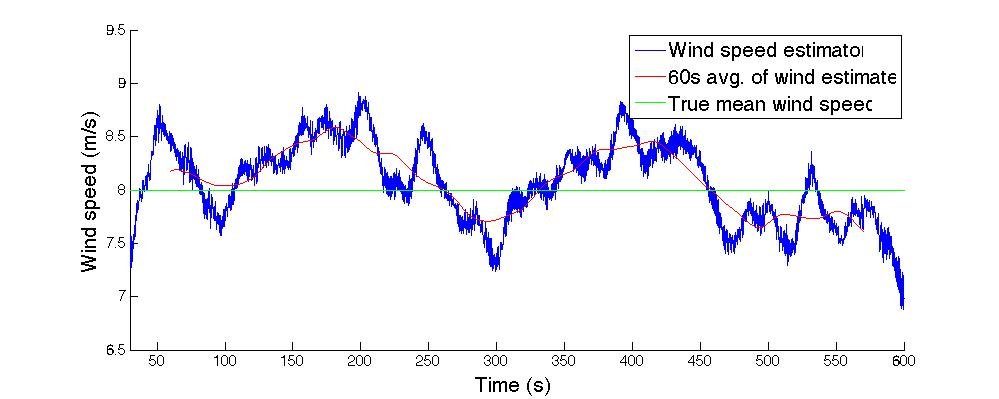
\includegraphics[width = \linewidth]{Figures/ch2Figures/fig2-25.jpg}
		
	\caption{Estimating $U_{mean}$ using a 60 s average of wind speed estimates for simulation \#13.}
	\label{fig2-25}
\end{figure}

By analyzing all of the test cases in our data set with a variety of averaging times we can create Figures \ref{fig2-26} and \ref{fig2-27}. These figures show the maximum and average discrepancies between the various averaged wind speed estimates and the known true mean wind speeds. In Figure \ref{fig2-26} we see that longer average times result in smaller mean discrepancies between the average wind speed estimate and the true mean wind speed. This is expected. Longer averaging times would likely perform even better, but 570 seconds was the longest averaging time we could use with the current data set. The highest mean discrepancies (as a \% of the true mean wind speed) are at low wind speeds. For some wind speeds (16 m/s - 22 m/s) Figure \ref{fig2-26} seems to show diminishing improvement for averaging times over 240 s. However, for the rest of the wind speeds Figure \ref{fig2-26} does not seem to show a clear point of diminishing returns.

Figure \ref{fig2-27} largely shows the same trends that we see in Figure \ref{fig2-26}, but the trends are a little less clear. Figure \ref{fig2-27} shows a few unexpected results. For example, in 18 m/s wind Figure \ref{fig2-27} an averaging time of 240 s gives a larger maximum discrepancy than any of the shorter or longer averaging times. I suspect that if we analyzed a lot more data some of these unexpected results would no longer be present.



\begin{figure}[ht]
	\centering
		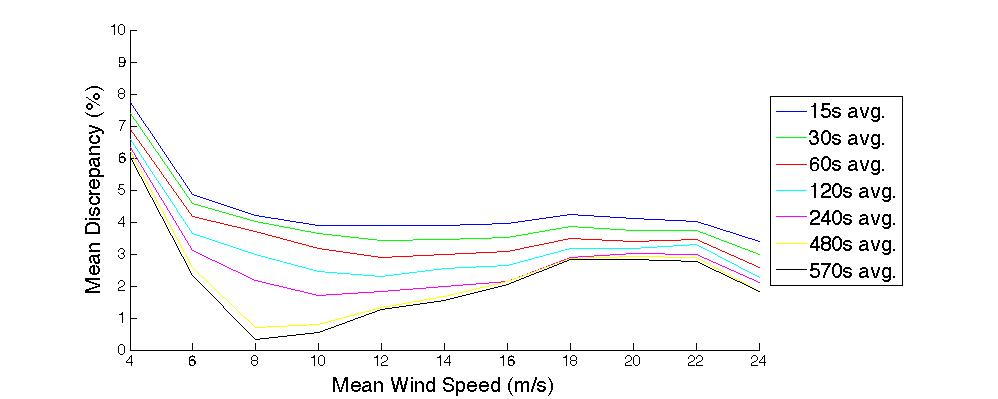
\includegraphics[width = \linewidth]{Figures/ch2Figures/fig2-26.jpg}
		
	\caption{Mean discrepency between true $U_{mean}$ and estimated $U_{mean}$ for a variety of averaging times.}
	\label{fig2-26}
\end{figure}

\begin{figure}[ht]
	\centering
		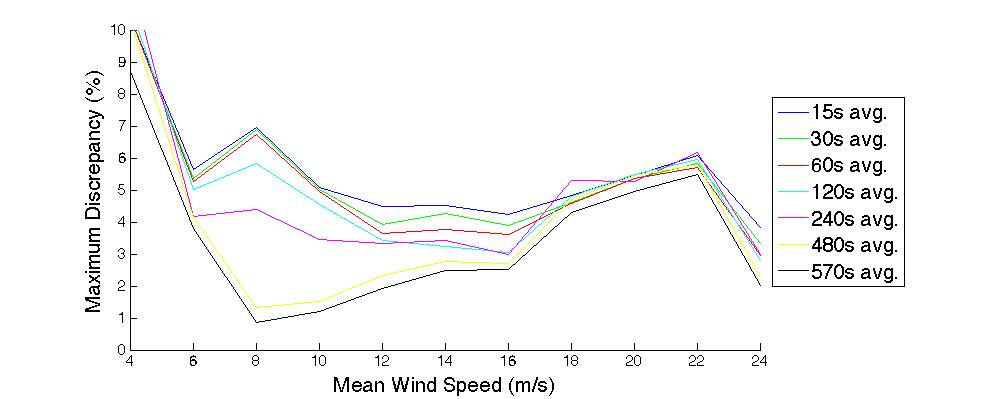
\includegraphics[width = \linewidth]{Figures/ch2Figures/fig2-27.jpg}
		
	\caption{Max discrepency between true $U_{mean}$ and estimated $U_{mean}$ for a variety of averaging times.}
	\label{fig2-27}
\end{figure}

Though Figures  \ref{fig2-26} and \ref{fig2-27} imply that the averaging time should be as long as possible, there is a practical reasons why a very long averaging time would be undesireable. When we simulate wind fields using TurbSim the mean wind speed remains constant, but research has shown that in real world conditions the mean wind speed does not remian constant indefinitely. In real world conditions the mean wind speed may be slowly changing \cite{vanderhoven1957}. If the mean wind speed is changing, we can minimize the impact on our wind speed averaging by keeping the averaging time short and by centering the averaging window on the time of interest. If we choose to center our averaging window on the time of interest, our averaging time is further constrained by the amount of time it will take wind speed fluctuations to propagate from the upwind turbine to the downwind turbine. For example, if the mean wind speed is 20 m/s and the downwind turbine is 1260 m (10$\times$ the NREL 5-MW rotor diameter) behind the upwind turbine, it will take about 63 seconds for the wind speed fluctuations to travel from the upwind turbine to the downwind turbine. In that scenario, the averaging time must be less than 126 seconds.

%-----------------------------------
%	SUBSECTION 5-1
%-----------------------------------
\subsection{A few thoughts on the limitations of Taylor's Frozen Turbulence Hypothesis}
Though Taylor$'$s hypothesis is often invoked in investigations of atmospheric turbulence, experimental results have shown that it is not universally accurate.  In particular, Taylor$'$s hypothesis is more accurate over short distances than over long distances and it is more accurate for low frequency wind speed fluctuations than high frequency fluctuations. \cite{higgins2012, schlipf2010}

%----------------------------------------------------------------------------------------
%	SECTION 6
%----------------------------------------------------------------------------------------

\section{Other Potentially Useful Turbine Sensors} \label{section2-6}

The methods discussed in previous sections aren't the only ways to use a turbine as a sensor for feed forward control. A typical turbine has other sensors that are potentially useful for feed forward control. This section briefly discusses two of those sensors, the wind vane and the rotor speed sensor.

Utility scale turbines are equipped with wind vane's that measure wind direction. Wind direction measurements are not used in this dissertation. The feed forward control schemes developed in Chapter \ref{Chapter3} and Chapter \ref{Chapter4} are simulated in a two turbine system where wind direction is treated as a known quantity. However, in a real world application of these feed forward control systems, wind direction measurements would be critical. In a wind farm each turbine would have many other turbines it could share information with. Wind direction would tell each turbine which other turbines it should send information to and which turbines it should receive information from. In many wind farms, wind direction changes seasonally or over the course of each day. As wind direction changes, wind vane readings would help the wind farm adapt and adjust how turbines share data for feed forward control.


Section \ref{section2-4} shows that rotor speed can be used with blade pitch and knowledge of turbine dynamics to estimate wind speed. However, rotor speed also has the potential to be useful on it's own. In region 3 control, the NREL 5-MW turbine attempts to track a constant rotor speed of 12.1 RPM. Any deviation from 12.1 RPM indicates a change in wind speed. Larger and/or more abrupt changes in wind speed result in larger deviations from 12.1 RPM. Since large abrupt changes in wind speed result in large structural loads on the turbine, there is a correlation between how much the rotor deviates from 12.1 RPM and how much gust induced structural loading the turbine experiences. Monitoring rotor speed could potentially be used as a simple way to identify the most damaging gusts. For example, a feed forward control system could consider anything causing a rotor speed over 13.31 RPM (10\% higher than the rated speed of 12.1 RPM) an extreme gust event. Whenever evidence of an extreme gust event is observed, the feed forward control system could take some kind of action to prepare downwind turbines for the gust.

%----------------------------------------------------------------------------------------
%	SECTION 7
%----------------------------------------------------------------------------------------

\section{Summary and Conclusions} \label{section2-7}

This chapter investigates ways to use a turbine as a sensor. The focus is on gathering data that could be useful for feed forward control. To ensure low cost, we only consider techniques that rely on sensors a modern utility scale turbine would already have.

Section \ref{section2-2} describes a set of 66 turbulent wind fields. Those wind fields are used in subsequent sections to evaluate sensor techniques. 

Section \ref{section2-3} discusses wind speed estimates based on nacelle top anemometer readings. First the limitations of anemometer measurements are discussed. Next, wind speed measurements at the rotor center are compared to the average wind speed over the rotor area. The discrepancies between those measurements are analyzed for the 66 turbulent wind fields described in Section \ref{section2-2}.
 
 Section \ref{section2-4} discusses wind speed estimates based on an inverted dynamic model of the turbine. The governing dynamic equations are derived. Those dynamic equations are then combined with WTPerf simulations of the NREL 5-MW turbine to develop a data sets that can be interpolated to estimate wind speed from tip speed ratio and collective blade pitch. Next, wind speed estimates based on turbine dynamics are compared to the average wind speed over the rotor area. The discrepancies between those measurements are analyzed for the 66 turbulent wind fields described in Section \ref{section2-2}. This wind speed estimation technique is found to provide more accurate wind speed measurements than the anemometer. The turbine dynamics based estimator has smaller average discrepancies and smaller maximum discrepancies with the average wind speed over the rotor area. Section \ref{section2-4-2} discusses the effect of yaw misalignment on turbine dynamics based wind speed estimation and how that effect could be compensated for. 
 
 Section \ref{section2-5} Discussed convection velocity and how to estimate it from wind speed estimates at a single location. 
 
 Section \ref{section2-6} discusses other turbine sensors, such as wind vanes or rotor speed sensors, that could be useful for feed forward control.